% Journal Article
% LaTeX Template
%-----------------------------------------------------------------------------
%	PACKAGES AND OTHER DOCUMENT CONFIGURATIONS
%-----------------------------------------------------------------------------

\documentclass[twoside,twocolumn]{article}

\usepackage{blindtext} % Package to generate dummy text throughout this template 

\usepackage[sc]{mathpazo} % Use the Palatino font
\usepackage[T1]{fontenc} % Use 8-bit encoding that has 256 glyphs
\linespread{1.05} % Line spacing - Palatino needs more space between lines
\usepackage{microtype} % Slightly tweak font spacing for aesthetics

\usepackage[english]{babel} % Language hyphenation and typographical rules
\usepackage{graphicx}
\usepackage{amsmath}
\usepackage{amssymb}
\DeclareMathOperator{\Tr}{Tr}
\usepackage[hmarginratio=1:1,top=32mm,columnsep=20pt]{geometry} % Document margins
\usepackage[format=plain, small,labelfont=bf,up,textfont=it,up]{caption} 
\usepackage{booktabs} % Horizontal rules in tables
\usepackage[format=plain, labelfont=bf,textfont=it]{subcaption}

\usepackage{lettrine} % The lettrine is the first enlarged letter at the beginning of the text
\usepackage{units}

\usepackage{xcolor} % adding color to words

\usepackage{braket} % braket notation

\usepackage{nameref} %to reference name of a section
\usepackage{hyperref}

\usepackage{enumitem} % Customized lists
\setlist[itemize]{noitemsep} % Make itemize lists more compact

\usepackage{abstract} % Allows abstract customization
\renewcommand{\abstractname}{\vspace{-\baselineskip}}
\renewcommand{\abstractnamefont}{\normalfont\bfseries} % Set the "Abstract" text to bold
% Set the abstract itself to small italic text
\renewcommand{\abstracttextfont}{\normalfont\small\itshape} 

\usepackage{titlesec} % Allows customization of titles
\renewcommand\thesection{\Roman{section}} % Roman numerals for the sections
\renewcommand\thesubsection{\roman{subsection}} % roman numerals for subsections
% Change the look of the section titles
\titleformat{\section}[block]{\large\scshape\centering}{\thesection.}{1em}{}
% Change the look of the section titles
\titleformat{\subsection}[block]{\large}{\thesubsection.}{1em}{}

\usepackage{fancyhdr} % Headers and footers
\pagestyle{fancy} % All pages have headers and footers
\fancyhead{} % Blank out the default header
\fancyfoot{} % Blank out the default footer
% Custom header text
\fancyhead[C]{Qiskit $\bullet$ April 2020} % $\bullet$ Vol. XXI, No. 1}
\fancyfoot[RO,LE]{\thepage} % Custom footer text

\usepackage{titling} % Customizing the title section
\usepackage{hyperref} % For hyperlinks in the PDF
\usepackage[page]{appendix}
\usepackage{pdfpages}
\renewcommand{\appendixpagename}{\vspace*{\fill}\centering Transpiled Circuits
\vspace*{\fill}}

% SI Units like the fancy Angstrom
\usepackage{siunitx}
\usepackage{bbold}

% Using BibTex, with specified choices of what to include in bibliography
\usepackage[backend=bibtex,
sorting=none, % sort entries by appearance
isbn=true,
doi=false,
url=true,
eprint=false,
abbreviate=false,
style=numeric]{biblatex}

% adding the bibliography file
\addbibresource{references}


%-----------------------------------------------------------------------------
%	TITLE SECTION
%-----------------------------------------------------------------------------

\setlength{\droptitle}{-4\baselineskip} % Move the title up

\title{\textbf{Quantum State Tomography and Post Measurement Analysis in Qiskit}} % Article title
\author{%
\textsc{Jerry Kamer, Roel van Silfhout, Nicholas Zutt}
\\[1ex]
\normalsize{Delft University of Technology}\\ % Your institution
}
\date{April 24, 2020} % Leave empty to omit a date
\renewcommand{\maketitlehookd}{%
\begin{abstract}
  \noindent The IBM Quantum Experience is a public platform for executing
quantum circuits on superconducting back-ends. We execute the Teleportation
protocol, Entanglement Swapping, Entanglement Purification and Grover's
Algorithm on three superconducting devices available from IBMQ. We present the
results using the appropriate post-measurement selection techniques and
reconstruct the output states through state tomography. We analyze the
performance of the three devices and put forth an explanation for the
discrepancies in the results between the three devices.
\end{abstract}


%%% Local Variables:
%%% mode: latex
%%% TeX-master: "report"
%%% End:
}

%-----------------------------------------------------------------------------

\begin{document}
	\maketitle

%-----------------------------------------------------------------------------
%	ARTICLE CONTENT
%-----------------------------------------------------------------------------

\section{Introduction}

\lettrine[nindent=0em,lines=3]{C} omputer simulations have arisen as powerful
tools for investigating the molecular dynamics of systems composed of
many particles. This report simulates the noble gas Argon at various temperatures
and densities, probing the three states of matter, and investigates a set of
macroscopic observables, the specific heat, pressure, pair correlation function
and diffusion constants of the system. \cite{nielsen10_quant}

In order to simulate a system of particles accurately, the first step is to
choose an appropriate potential with which to model the inter-atomic forces
exchanged between the particles in motion. We use a mathematically simple model
that has been popular historically due to its computational efficiency and which
has the added benefit of being especially accurate for noble gases. It assumes
dipole-dipole interaction between neutral atoms, and includes a repulsive term
for short distances. This is the Lennard-Jones potential, which has the form


%%% Local Variables:
%%% mode: latex
%%% TeX-master: "report"
%%% End:


\section{Theory}
In a classical computer its internal state is measured at different points in time in order to debug the system. However, for a quantum computer, the analogy would be the measurement of its density matrix, which is called state tomography. We first define the density matrix of a single qubit,
\begin{equation}
\rho=\frac{1}{2}\left(I+\sum_i\alpha_i\sigma_i\right)
\end{equation}
where $\sigma_i$ are all the Pauli-matrices and $\alpha_i$ are the real-valued coefficients. Using the trace orthogonality of the Pauli-matrices,
\begin{equation}
\Tr\left(\sigma_j\sigma_k\right)=2\delta_{jk}
\end{equation}
we can derive the real-valued coefficients by calculating the expectation values of the different Pauli-matrices.
\begin{equation}
\Tr\left(\rho\sigma_i\right)=\left\langle\sigma_i\right\rangle=\alpha_i
\end{equation}
By measuring the single qubit in the different basis (X,Y and Z) we can derive these expectation values. This requires a repeated preparation and measuring of the final state. In reality, the measured expectation values are estimations of $\left\langle X\right\rangle,\left\langle Y\right\rangle,\left\langle Z\right\rangle$. Often in a quantum computer the measurements are only done in the $Z$-basis. Other operators are realized using rotation operators before the final measurement.

In order to convert the estimated- to real expectation values we correct for readout error, which will give us a better estimation of the density matrix $\rho$. If $\epsilon_{10},\epsilon_{01}$ are the probabilities that a $\left|0\right\rangle$ state gives an eigenvalue back of -1 and a $\left|1\right\rangle$ state which is measured as a eigenvalue 1, and if $\alpha,\beta$ are coefficients of the final state $\left|\psi\right\rangle$, then the measured expectation value $\left\langle m\right\rangle$ in the $Z$-basis is
\begin{equation}
\left\langle m\right\rangle=\left(1-\epsilon_{10}\right)\left|\alpha\right|^2+
\end{equation}





  

\section{Devices}

Superconducting qubits are constructed macroscopic circuits which nonetheless
exhibit quantum behaviour. They consist of an inductor $L$ connected to a
capacitor $C$. These are described by the equations of motion of a harmonic
oscillator, with flux $\phi$ through the inductor playing the role of the
canonical position which oscillates out of phase with the charge $Q$ on the
capacitor, this charge playing the part of the canonical momentum
\cite{devoret04_implem_qubit_with_super_integ_circuit}. This LC oscillator has a
resonance frequency that can be specifically engineered as it is given by
$\omega_0 = \nicefrac{1}{\sqrt{LC}}$, and which typically comes in the microwave
frequency range for our qubits. The superconducting nature of the oscillator is
of critical importance to maintaining coherence as a superposition of the ground
and first excited states of the LC oscillator decays on a time scale given by
$\nicefrac{1}{RC}$, where $R$ is the resistance. LC circuits, as macroscopic
qubits, are attractive partly because their parameters can be engineered to
whatever values best suit the needs in question, but it should be noted that
their size also entail some individuality to each qubit that may lead to
variations in their functioning.

\begin{figure}[h] \centering
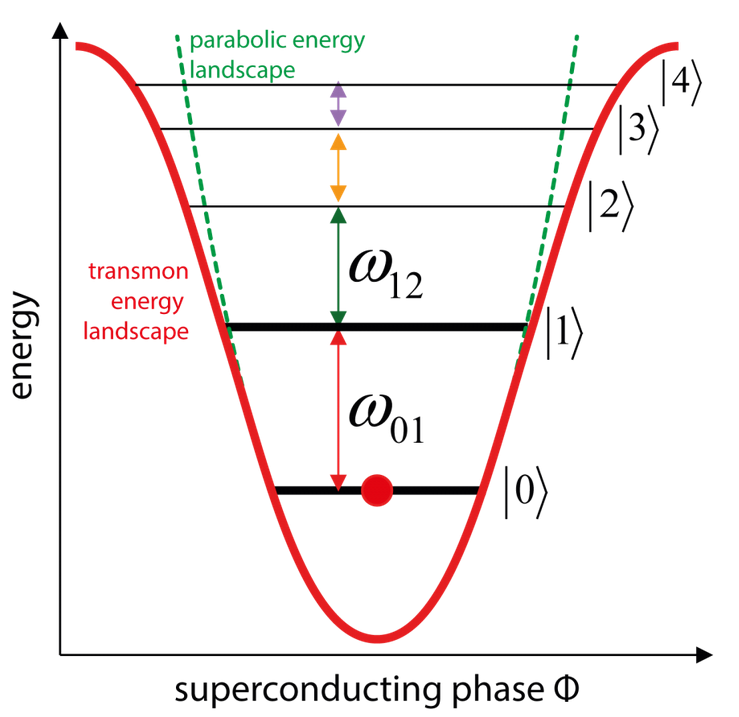
\includegraphics[width=0.48\textwidth]{images/energy_spacing_transmon.png}
  \caption{The energy spacing between levels of an LC oscillator are ordinarily
even, anharmonicity, introduced through the inclusion of a Josephson tunnel
junction, splits the level spacing. Figure from
\cite{dickel20_how_to_make_artif_atoms}.}
  \label{fig:energy_spacing_transmon}
\end{figure}

A simple LC circuit alone, though, cannot be an effective qubit. Its quantized
energy levels come evenly spaced, which means that driving between one
transition (say from $\ket{0}$ to $\ket{1}$) drives between \textit{all}
transitions \cite{devoret04_implem_qubit_with_super_integ_circuit,
Devoret2004SuperconductingQA}. In order to be able to control the qubit state
effectively, the transition frequency between the states $\ket{0}$ and $\ket{1}$
has to be different enough from all other transitions, but of course, all
transitions between neighbouring states in the harmonic oscillator potential are
the same size. A degree of anharmonicity is then brought in by a Josephson
tunnel element with its own non-linear inductance which is added to the circuit
in parallel with the capacitor, replacing the inductor and making it possible to
individually drive transitions between specific levels in the LC oscillator, as
shown in Fig. \ref{fig:energy_spacing_transmon}. The system's dynamics can then
be effectively confined to just the two lowest energy levels as long as the
driving frequency for transitions are properly tuned
\cite{devoret04_implem_qubit_with_super_integ_circuit}.

\begin{figure}[h] \centering
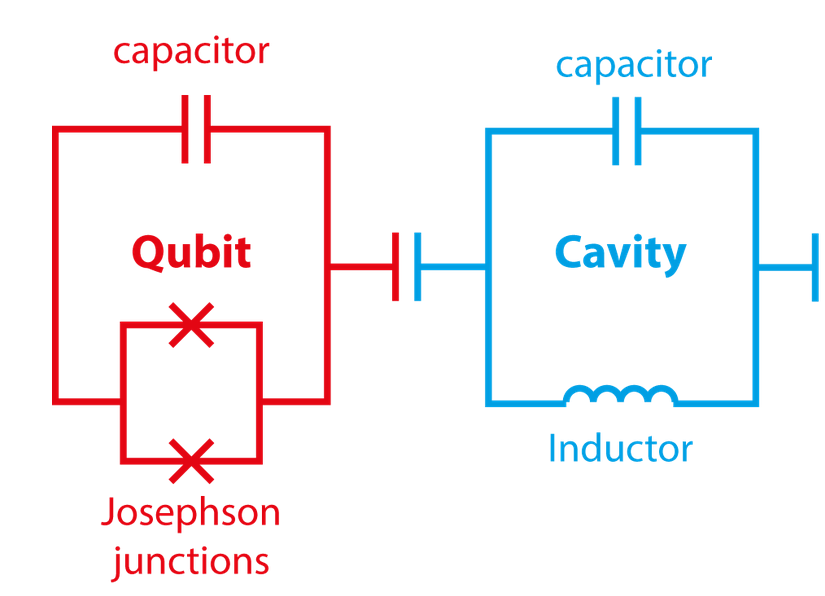
\includegraphics[width=0.48\textwidth]{images/transmon_diagram.png}
  \caption{A schematic of a transmon qubit. The left superconductor maintains
anharmonicity while the right superconductor helps protect it from charge noise.
Figure from \cite{dickel20_how_to_make_artif_atoms}.}
  \label{fig:transmon}
\end{figure}

The devices at the IBM Quantum Experience are transmon qubits. This type of
superconducting charge qubit, shown in Fig. \ref{fig:transmon}, consists of a
qubit circuit coupled to a cavity circuit (a harmonic LC oscillator) which has a
reduced sensitivity to charge noise and has recently shown coherence times of up
to 95$\mu$s and relaxation times of around 70$\mu$s.
\cite{koch07_charg_insen_qubit_desig_deriv,
rigetti12_super_qubit_waveg_cavit_with}. Three devices at the IBM Quantum
Experience were chosen to be used in this project. In the following section we
will provide an overview of these devices to give context for the results
that will be discussed below. IBM names its superconducting devices after major
cities, and those we are interested in are code-named Burlington, Melbourne and
Yorktown.

\subsection{Specifications}\label{Specifications} When comparing the different backends, the first
parameters to take into account in their characterization is the error rates for
single- and two-qubit operations. All three backends use the same universal gate
set, which make their error rates directly comparable. As can be seen in Fig.
\ref{fig:burlington_connections}, the Burlington backend has the best gate error rates of
any backend we will consider, with a single-qubit U2 error rate less than
0.065\% for all qubits and a CNOT error rate of less than 1.645\%.

\begin{figure}[h] \centering
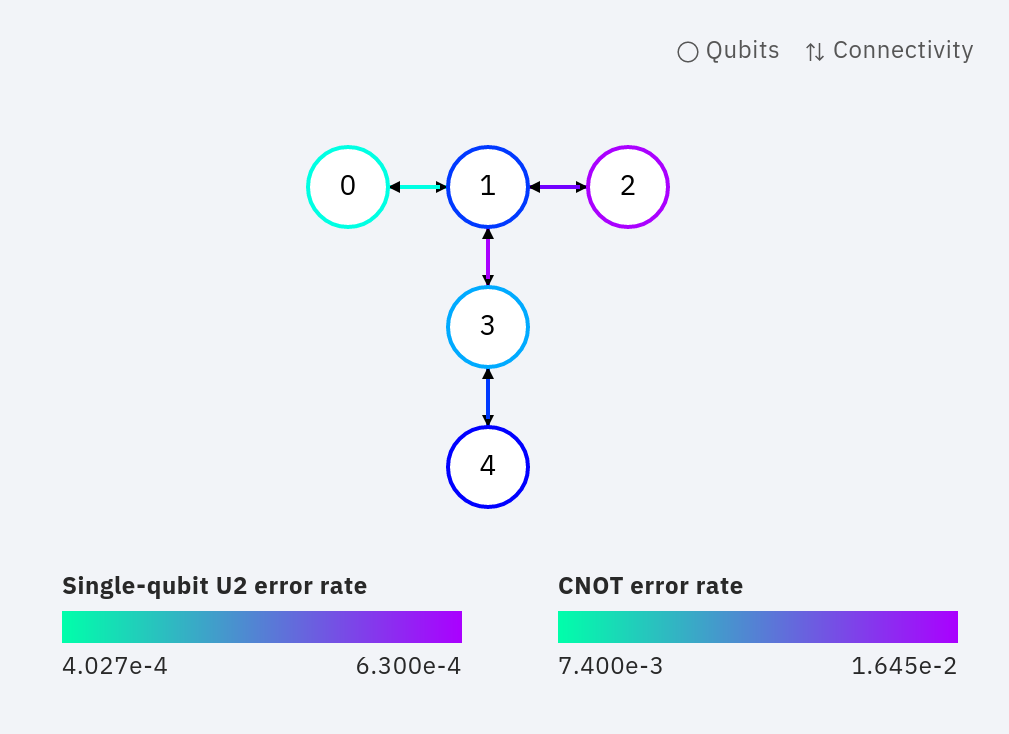
\includegraphics[width=0.48\textwidth]{images/connection_diagram_burlington.png}
  \caption{The T-shaped Burlington device. Though the device has relatively
small error rates, the limited connectivity plays a big role in the device's
performance, as many extra gates are needed to implement circuits when there are
few direct connections. Figure from \cite{ibmq_burlington}.}
  \label{fig:burlington_connections}
\end{figure}

In the Melbourne backend (Fig. \ref{fig:melbourne_connections}), single-qubit
gate errors rise to 0.746\%, though the qubits used in all the circuits
implemented here (qubits numbered 0, 1, 2 and 14) all have errors under 0.07\%.
CNOT error between the four qubits of interest to our circuits stays below 4\%.
When choosing which qubits to use for computation, the transpiling program seems
to favour implementation on qubits with the lowest errors (hence the avoidance
of the noisy qubit 13).

The individual character of the qubits is most easily seen in the Melbourne
device. Due to variability in the manufacture of the macroscopic qubits, some
come out noisier than others, and the connections between them likewise suffer
some in-homogeneity.
\begin{figure}[h] \centering
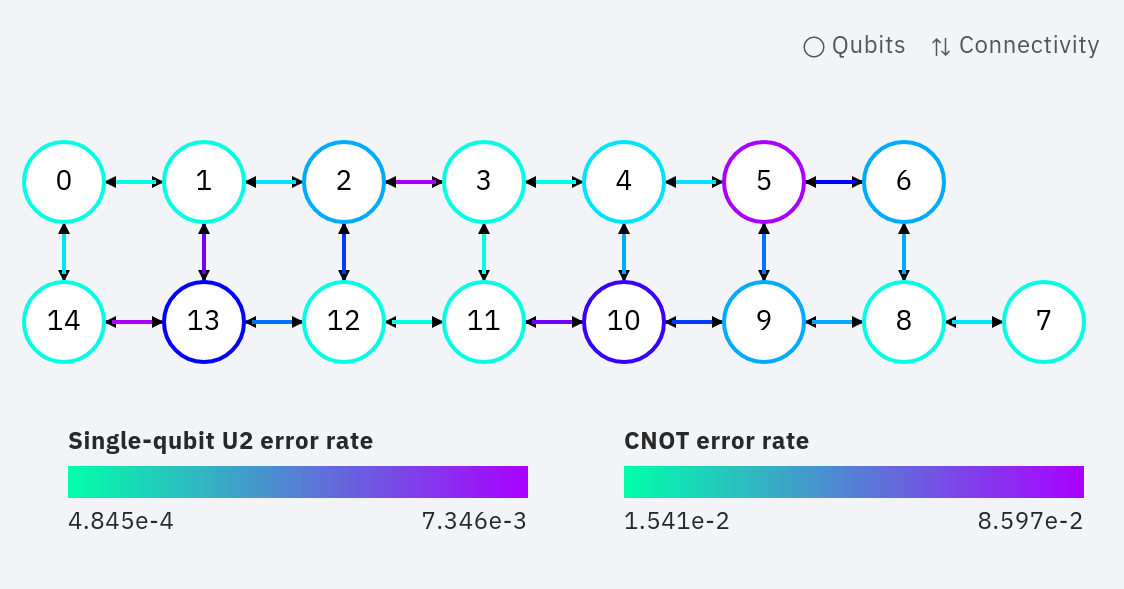
\includegraphics[width=0.48\textwidth]{images/connection_diagram_melbourne.png}
  \caption{The largest publicly available device at IBM Q. The individual
character of the transmons is visible in this diagram through the large
variability in the error rates. Figure from \cite{ibmq_16_melbourne}.}
  \label{fig:melbourne_connections}
\end{figure}

The final backend under consideration, shown in Fig.
\ref{fig:yorktown_connections} comes out between Melbourne and Burlington with
an average single-qubit error rate of 0.05\% and average CNOT error of 2.276\%.
However, as we will see in the results, these gate error rates are far from the
whole story when it comes to explaining the performance of various backends.
\begin{figure}[h] \centering
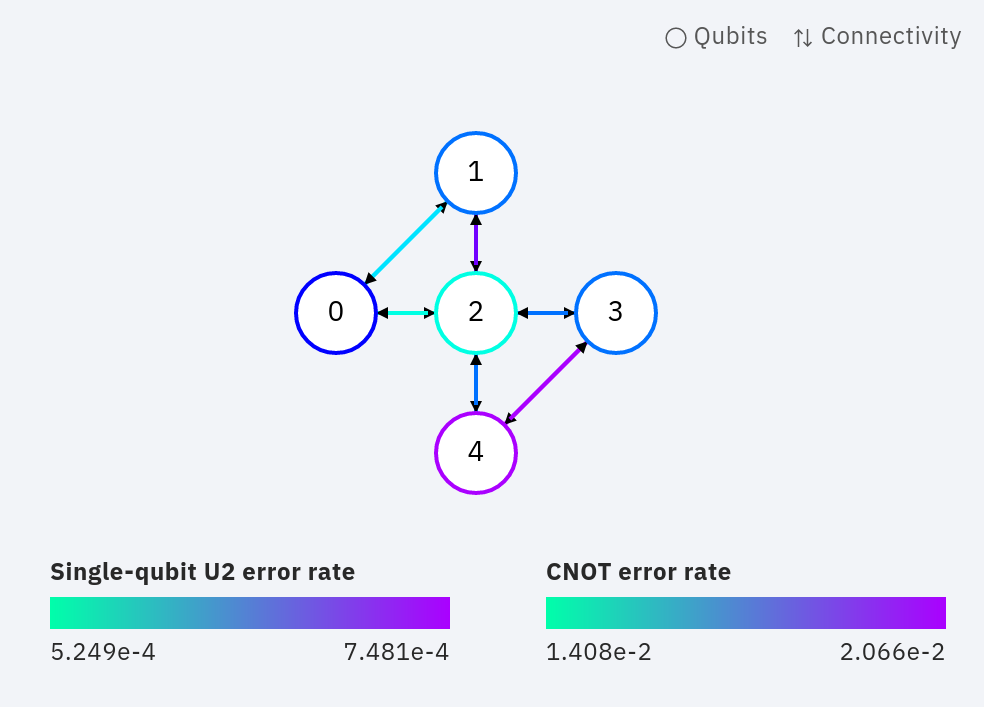
\includegraphics[width=0.48\textwidth]{images/connection_diagram_ibmqx2.png}
  \caption{The most densely connected 5-qubit device at IBM Q. As we will see,
equally as important as the single-qubit and CNOT error rates is the degree of
connectivity in a device. Figure from \cite{ibmq_yorktown}.}
  \label{fig:yorktown_connections}
\end{figure}

\begin{table} \centering
	\begin{tabular}{lrrrr} \toprule Backend & $U_2 (\%)$ & $CNOT (\%)$ \\ \midrule
		Burlington & 0.050 & 1.213 \\ Melbourne & 1.258 & 2.156 \\ Yorktown & 0.689 &
		2.275 \\ \bottomrule
	\end{tabular}
	\caption{Average percent error on single-qubit $U_2$ gates and CNOT gates for
		the three devices used to implement the circuits of interest. All averages taken
		from data provided at \cite{ibmq_burlington,ibmq_16_melbourne,ibmq_yorktown}.}
	\label{tb:average_errors}
\end{table}
One consideration that is not reflected in the gate error rates which has a
significant impact on the fidelity of the outputs of circuits is the number of
direct connections between qubits. Burlington may have the lowest average error
rates for gate operations of all the three devices (shown in Table
\ref{tb:average_errors}), but as we will show, this doesn't translate to better
output fidelities in every case. In fact, because the number of gates required
to implement each circuit will vary from device to device, the optimal backend
on which to conduct a given computation will ultimately depend more on the
configuration of each backend, rather than gate errors.

%%% Local Variables:
%%% mode: latex
%%% TeX-master: "report"
%%% End:

\section{Quantum Circuits}
\label{sec:circuits}
For this research we have chosen to execute the Teleportation protocol, Grover's
search algorithm, Entanglement Swapping and Entanglement Purification on the
devices. The circuits are all made using an open source software development kit
called Qiskit, which uses Python as its main programming language. The written
codes, made with Jupyter Notebook, for the circuits can be found in the \hyperref[apen]{appendix}. In the following we will describe the circuits,
mainly focussing on the states and the measurements.
Thereafter, a summary of the execution of a code will be given.

\subsection{The Teleportation protocol}
\label{sub:tele}
Quantum teleportation is a procedure where a quantum state can be transmitted
from one location to the other. Usually this is done by creating an arbitrary
state $\ket{\psi}$ on the first qubit and a $\ket{\Phi^+}$ Bell-state on the
second and third qubit, as can be seen in figure \ref{fig:telgen}.

\begin{figure}[h]
  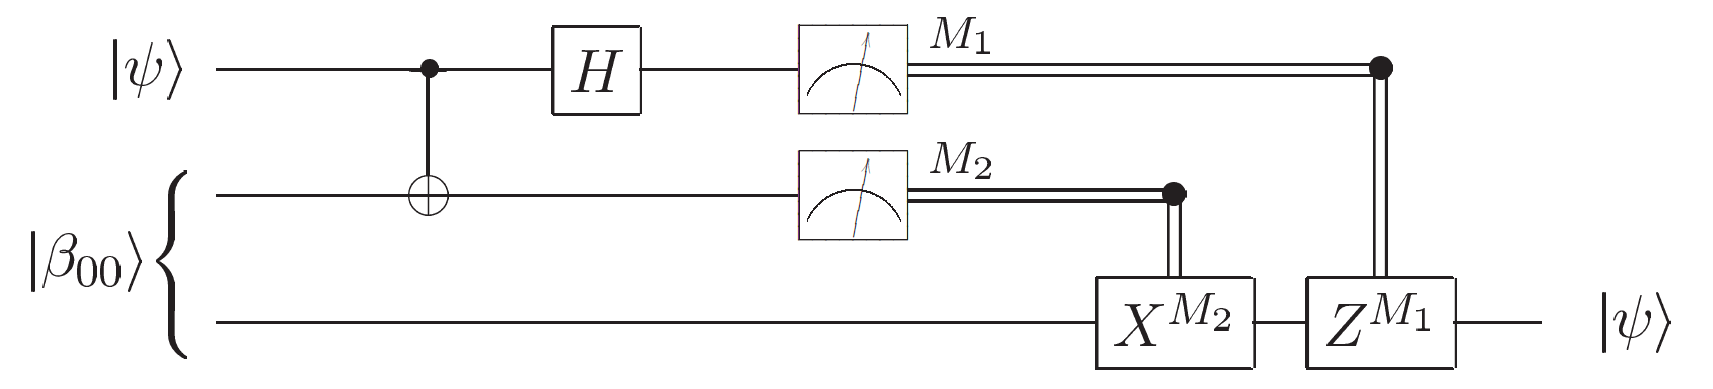
\includegraphics[width=0.48\textwidth]{images/Teleport_general.png}
	\caption{General teleportation protocol circuit. Here the $\ket{\Phi^+}$
Bell-state is denoted as $\ket{\beta_{00}}$. \cite{nielsen10_quant}}
	\label{fig:telgen}
\end{figure}

Subsequently, a CNOT gate is applied to the second qubit and a
Hadamard gate to the first qubit. Now the first and second qubit will be
measured in the Z-basis, with the measurement results being $M_1$ and $M_2$,
respectively. A X- and/or Z-gate is applied to the third qubit depending on the
measurement outcome. If $M_1 = -1$ a Z-gate will be applied and if $M_2 = -1$ a
X-gate will be applied. This will result in the state $\ket{\psi}$ being
teleported to the third qubit.

However, to know if the state $\ket{\psi}$ is properly transported, the third
qubit must be measured. Unfortunately, it is not possible (yet) to apply a gate
after a measurement on the used devices. So, we will have to resort to post
measurement techniques, as the gates cannot be applied to the third qubit. The
circuit that is send to the devices is presented in figure \ref{fig:telcir}.

\begin{figure}[h]
  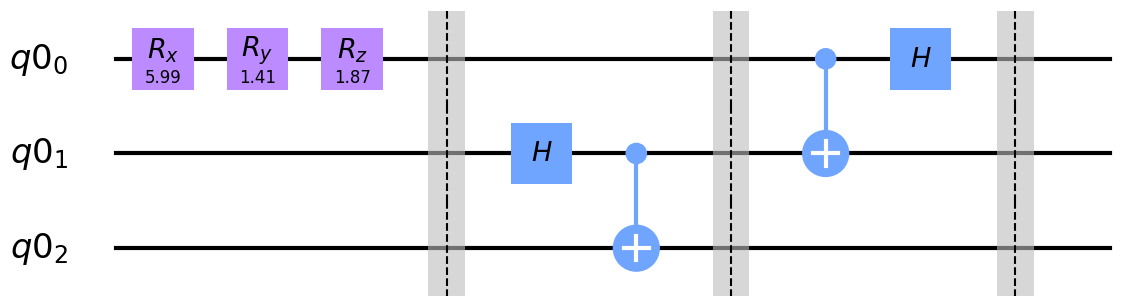
\includegraphics[width=0.48\textwidth]{images/teleport_circuit.png}
	\caption{Teleport circuit used for the measurements. (The operators on the
first qubit are randomized every run.)}
	\label{fig:telcir}
\end{figure}

As one can easily see the gates on the third qubit are absent. To
account for this, a Pauli-X or Pauli-Z matrix is applied to the final state on
the third qubit, after the measurement. Which works similar to the general
protocol: if $M_1 = -1$ a Pauli-Z matrix will be applied and if $M_2 = -1$ a
Pauli-X matrix will be applied. This will, in post measurement, result in the
state $\ket{\psi}$ being teleported to the third qubit.

\subsection{Grover's search algorithm}
The Grover search algorithm can find an input given to a black box with a high
likeliness. In our case, the input that is given is a unitary 4x4 diagonal
matrix, with three values being +1 and one being -1. The algorithm can find
which one of the numbers on the diagonal is -1. The circuit that is used in the
measurements is presented in figure \ref{fig:grocir}.
\begin{figure}[h]
  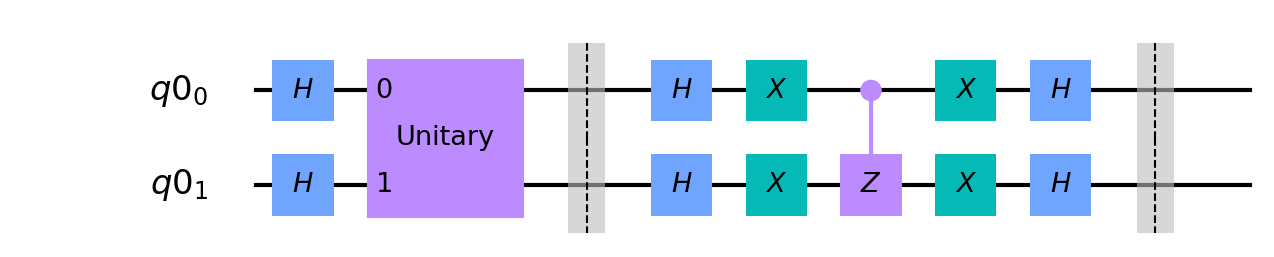
\includegraphics[width=0.48\textwidth]{images/grover_circuit.png}
	\caption{Grover's search algorithm circuit used for the measurements. (The
position of the -1 value is randomized every run.)}
	\label{fig:grocir}
\end{figure}
For explanatory reasons, let us choose the unitary matrix to be:
\begin{equation*} U =
  \begin{bmatrix}
    1 & 0 & 0 & 0 \\
    0 & 1 & 0 & 0 \\
    0 & 0 & 1 & 0 \\
    0 & 0 & 0 &-1
\end{bmatrix}
\end{equation*}
$U$ is randomized for every run of the circuit on a device or
simulator. The two qubit will both start in the $\ket{0}$ state. After the
application of the Hadamard gates the total state will be: $\ket{\Psi} =
\frac{1}{2}\left(\ket{00}+\ket{01}+\ket{10}+\ket{11}\right)$. Now $U$ is applied
giving: $\ket{\Psi} =
\frac{1}{2}\left(\ket{00}+\ket{01}+\ket{10}-\ket{11}\right)$. The part after the
unitary in figure \ref{fig:grocir} is important for the Grover's search
algorithm and does an inversion about the mean. This inverts the constants
multiplied with each state around the mean of the total. In this case the mean
is $\frac{3\cdot\frac{1}{2}-\frac{1}{2}}{4} = \frac{1}{4}$. Inverting
$\frac{1}{2}$ about the mean, means that it will become 0. For $-\frac{1}{2}$ it
will become 1, thus making $\ket{11}$ the only state left. Measuring this will
result in $M_1 = M_2 = -1$. This result is related to where in $U$ the -1 value
is positioned and in this case the result shows it is in the bottom right corner
(where we positioned -1 in the first place).

\subsection{Entanglement swap}
This protocol is, as the name states, a way of changing the entanglement between two qubits, for example the first and second, to an entanglement between different qubits, for example the first and fourth. This circuit will first be generally described, and can be found in figure \ref{fig:swapgen}.
\begin{figure}[h]
	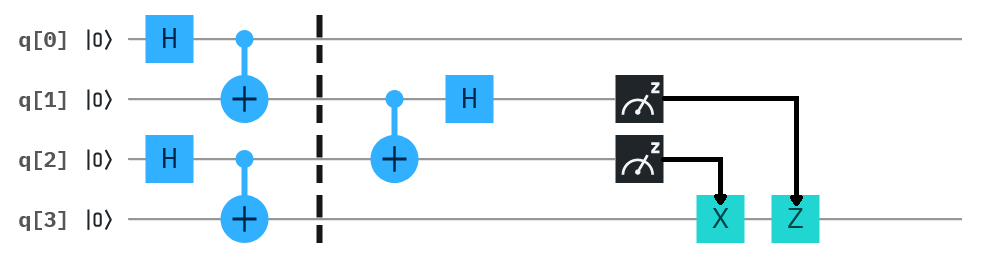
\includegraphics[width=0.48\textwidth]{images/swap_general.png}
	\caption{General entanglement swap protocol circuit. Made using the IBM Quantum experience Circuit Composer.}
	\label{fig:swapgen}
\end{figure}

First, an arbitrary Bell-like state is created on the first two qubits (q[0] and q[1]). For explanatory reasons, this is now a simple $\ket{\Phi^+}$ Bell state. On the third and fourth qubit, a $\ket{\Phi^+}$ state is also created. This gives the following state: $\ket{\Psi} = \frac{1}{2}\left(\ket{0000}+\ket{0011}+\ket{1100}+\ket{1111}\right)$. So at this point our arbitrary state has entanglement with the first and second qubit, which are the fourth and third number in de bra-ket notation, respectively. Now, a CNOT gate is applied between the second and third qubit resulting in: $\ket{\Psi} = \frac{1}{2}\left(\ket{0000}+\ket{0111}+\ket{1100}+\ket{1011}\right)$. After the application of the Hadamard gate to the second qubit we get eight different possible states: 
%Did something weird with the equation here or else it wouldn't fit in the text
$\ket{\Psi} = \frac{1}{\sqrt{8}}(\ket{0000}+\ket{0010}+\ket{0101}-\ket{0111}+\ket{1001}$$-\ket{1011}+\ket{1100}+\ket{1110})$. Now for the measurement part. If the result would be $M_1 = +1$ and $M_2 = -1$, a X-gate is applied to the fourth qubit. This would result in: $\ket{\Psi} = \frac{1}{\sqrt{2}}\left(\ket{0100}+\ket{1101}\right)$. One can see that the first and fourth qubit now have the combined state $\frac{1}{\sqrt{2}}\left(\ket{00}+\ket{11}\right) = \ket{\Phi^+}$, so the entanglement is swapped from the first and the second to the first and the fourth qubit.

However, we have to resort to post measurement techniques. Already stated in the \hyperref[sub:tele]{teleportation protocol} section, gates cannot be applied after
measurement. The circuit that is given to the devices and simulators is shown in
figure \ref{fig:swapcir}.
\begin{figure}[h]
	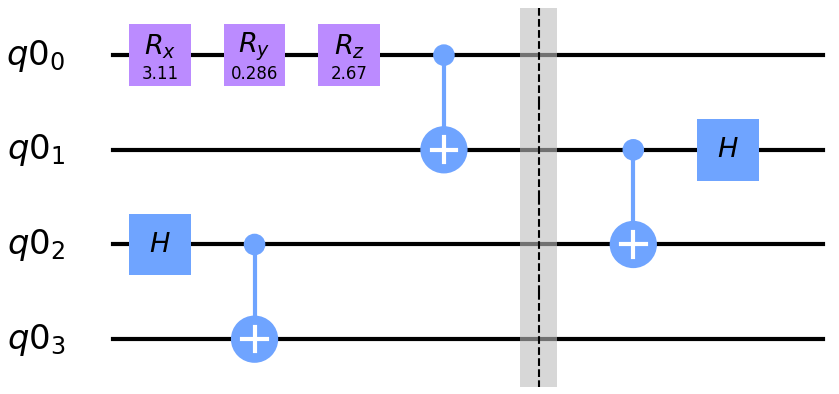
\includegraphics[width=0.48\textwidth]{images/swap_circuit.png}
	\caption{Entanglement swap circuit used in the measurements. Every measurement a random Bell-like state is created on the first two qubits.}
	\label{fig:swapcir}
\end{figure}
At the beginning of every measurement, a random Bell-like state is created. Now, the circuit runs identical to what is explained before, till the measurements take place. After the measurement, a Pauli-X or Pauli-Z matrix is applied to the fourth qubit. This depends on the measurement outcome of $M_1$ and $M_2$. If $M_1 = -1$ we apply a Pauli-Z matrix and if $M_2 = -1$ we apply a Pauli-X matrix. This will give, excluding any errors, an entangled state (post measurement) which we can use for our calculations and comparisons.

\subsection{Entanglement purification}
The entanglement purification is a very useful protocol that ensures a final state is a $\ket{\Phi^+}$ Bell state when the input state is not a perfectly entangled Bell state. This circuit is shown in figure \ref{fig:purcir}. Also, this is the circuit that is used on the devices for measurements.
\begin{figure}[h]
	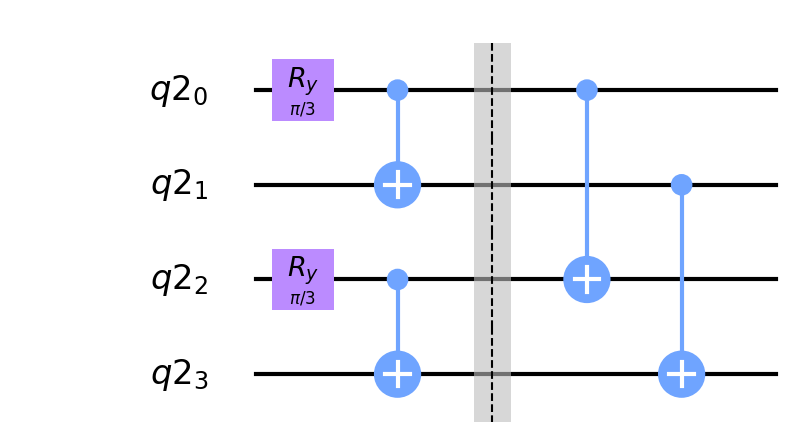
\includegraphics[width=0.45\textwidth]{images/purification_circuit.png}
	\caption{Entanglement purification circuit used in the measurements. The rotation at the beginning of the circuit can be determined using an input fidelity, $F$. In this case $F = 0.75$.}
	\label{fig:purcir}
\end{figure}

First, the circuit makes a not perfectly entangled Bell state by rotating the first and third qubit a certain angle, $\theta$, around the y-axis and subsequently applying a CNOT gate to the first and second and the third and fourth qubit. This angle is determined by a chosen input fidelity, $F$. In this case $F = 0.75$. Later will be explained how this translates to an angle. This will result in the state $\ket{\Psi} = 0.933\ket{0000}+0.067\ket{1111}+0.250\left(\ket{0011}+\ket{1100}\right)$. Now a CNOT gate is applied to the first and third qubit giving: $\ket{\Psi} = 0.933\ket{0000}+0.067\ket{1011}+0.250\left(\ket{0111}+\ket{1100}\right)$. Thereafter, another CNOT gate is applied to the second and fourth qubit: $\ket{\Psi} = 0.933\ket{0000}+0.067\ket{0011}+0.250\left(\ket{1111}+\ket{1100}\right)$. An important part of this circuit is that the bottom two qubit measurements must give -1 as this will ensure that the state of the top two qubits becomes $\ket{\Psi_{1,2}} = \frac{1}{\sqrt{2}}\left(\ket{11}+\ket{00}\right) = \ket{\Phi^+}$. In this case the probability for measuring this would be $2\cdot0.250^2 = 0.125$. For other input fidelities, the probability would ofcourse be different. One could argue that a measurement of +1 for both bottom qubits also gives a Bell state, but this state would not have the same factors, so it will not be perfectly entangled. In the measurements we account for this by only fabricating density matrices for the results where the bottom two qubits measurements where -1.

Generally a not perfectly entangled $\ket{\Phi^+}$ state can be described by the following $\ket{\psi} = \cos{\frac{\theta}{2}}\ket{00} + \sin{\frac{\theta}{2}}\ket{11}$, in which $\theta$ is the angle of rotation along the y-axis. The density matrix of this state, $\rho$, can be calculated as 
$\rho = \ket{\psi}\bra{\psi} = \cos^2{\frac{\theta}{2}}\ket{00}\bra{00} + \cos{\frac{\theta}{2}}\sin{\frac{\theta}{2}}\left(\ket{00}\bra{11}+\ket{11}\bra{00}\right)+\sin^2{\frac{\theta}{2}}\ket{11}\bra{11}$. 
The fidelity with respect to the $\ket{\Phi^+}$ state is defined as: $F = \bra{\Phi^+}\rho\ket{\Phi^+}$. Filling in $\rho$ and calculating $F$ will result into $F = \frac{1}{2}\left(1+\sin{\theta}\right)$, which can be rewritten to have $\theta\left(F\right) = \arcsin{\left(2F-1\right)}$. In our case, for $F = 0.75$, the rotation angle $\theta$ would become $\theta = \frac{\pi}{6}$.

\subsection{Code execution}
The circuits are build using Qiskit, a very user friendly open source software that lets the user make quantum circuits and execute them on simulators or devices. IBM their devices are easily implementable in the executions using Qiskit, which gave us the easy choice for using their devices for circuit execution. In the following a concise summary will be given of what steps are taken in the codes for the different circuits. We advise the reader to also have one of our codes visible while reading the summary.

Starting off, the proper modules are imported in the code. One must think about modules for circuit building, visualization, tomography calculations, measurement calibrations, etcetera. Secondly, the IMBQ device needed for the calculation is selected. In order to use the devices, one must have an account at IBM Quantum Experience, where one can get a token which gives (limited) access to their devices. Also, the necessary preparations for the noise calculation are done. As we would like to do a noise simulation using the noise model for the chosen device, this must be properly selected as well. Next, the required circuit is build and visualized, both generally and for the device. An expected state is created from the circuit. This means the state we would expect without any error in the circuit. For the circuits with a Bell-like states, the expected state of the $\ket{\Phi^+}$ is created. This all is done for future fidelity calculation. Subsequently, the measurement readout correction is performed, which is a build in function in Qiskit. This function does a measurement for only certain gates on a empty circuit. Since we are only interested in one or two qubits, we first select which are relevant for our study. For example, the entanglement purification circuit only requires correction on the top two qubits. This is executed on the device 8,192 times (shots). The results are processed accordingly to get the $B$ matrix and $\vec{\beta}$ vector. Next, the tomography circuits are send to the simulator, noise simulator and the device. These are nine circuits which have a combination of a Hadamard and/or S$^\dagger$-gate before the measurements of the relevant qubits. As before, these have 8,192 shots as well. After the runs, the results are used to make full states in all the possible basis.
 
These full states are then used for the calculation of the density matrices. During this calculation, measurement readout correction and post measurement techniques are also applied. For example, only keeping the data which has $\ket{11}$ as the state for the bottom two qubits in entanglement purification. Using the density matrices acquired from the three runs, the fidelities are calculated by comparing the resulting matrices to the expected one created at the beginning. The execution of the circuits is repeated 15 times, giving a total of 122,880 shots per device.

%%% Local Variables:
%%% mode: latex
%%% TeX-master: "report"
%%% End:


\section{Results} In the following sections we will discuss some key results;
for a more complete look at the output of the scripts, we ask that you please
consult the Appendices.

\subsection{Teleportation} The main result of the teleportation protocol is
summarized in Fig. \ref{fig:teleport_histogram}. The ideal simulation fidelities
are all within statistical error of unity, an important check to ensure that the
state, reconstructed through tomography, and post-measurement selection scheme
both are working as expected. The Noisy Simulator is modelled using the
single-qubit errors, CNOT errors and a model of readout error in each backend
\cite{qiskit_org}. As we will continue to see with the other circuits, the noise
model overestimate the performance of the backend, but interestingly in this
case, for the Melbourne device, we find that the noise model almost matches that
of the device.

The noise model captures the error in the Burlington device much less
accurately. We would expect that Burlington would perform almost as well as
Yorktown from the estimates on the noisy simulator, but in fact it performs the
worst of the three. We suspect, as will be described in more detail below, that
this is a consequence of the number of gates needed to implement the circuit on
the real device.

\begin{figure}[h] \centering
	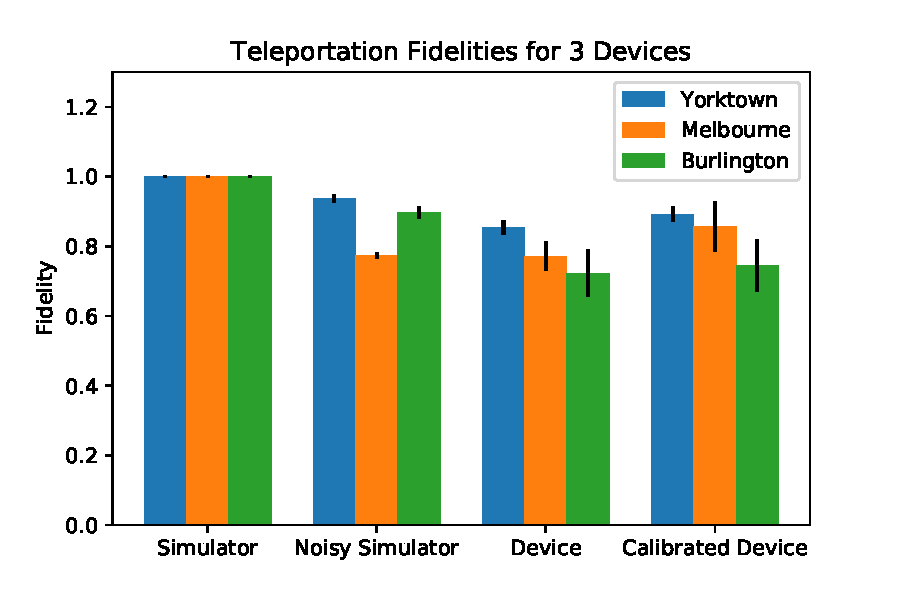
\includegraphics[width=0.48\textwidth]{images/results/teleport_histogram.pdf}
	\caption{Fidelity results for the Teleportation protocol. Error bars are
		estimated by taking the variance over 15 runs of 8,192 shots each (a total of
		122,880 shots). All simulation fidelities are within statistical error of
		unity.}
	\label{fig:teleport_histogram}
\end{figure}
In order to check the readout calibration, it is useful to compare Pauli sets of
the different outcomes, which we can see in Fig. \ref{fig:tele_paulis}.
\begin{figure}
  \begin{subfigure}{.5\textwidth} \centering % include first image
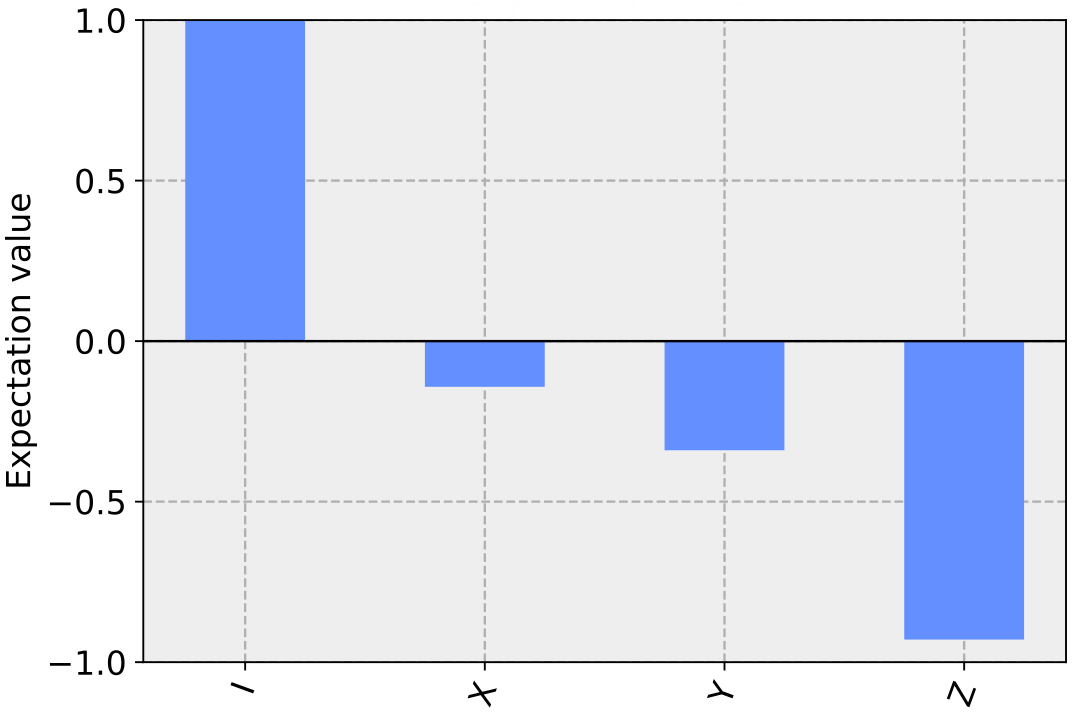
\includegraphics[width=.8\linewidth]{images/results/tele_pauli_sim.png}
    \caption{The expected Pauli set.}
    \label{fig:tele_pauli_sim}
  \end{subfigure} \newline
  \begin{subfigure}{.5\textwidth} \centering % include second image
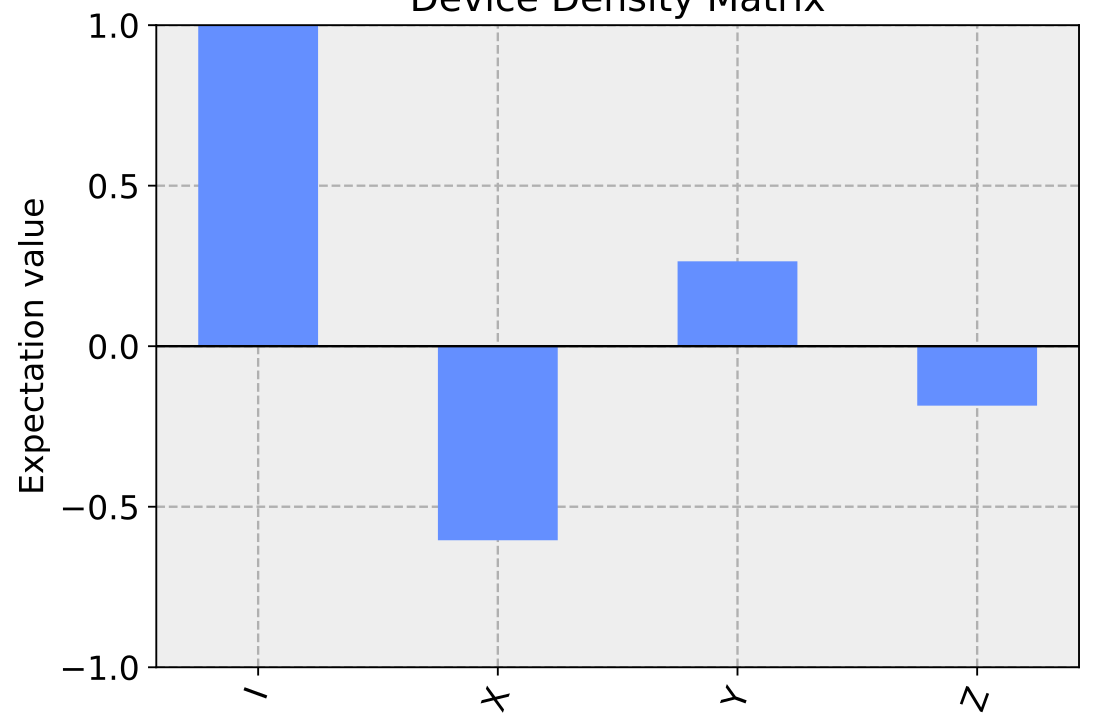
\includegraphics[width=.8\linewidth]{images/results/tele_pauli_dev.png}
    \caption{The output Pauli set for the device.}
    \label{fig:tele_pauli_dev}
  \end{subfigure} \newline
  \begin{subfigure}{.5\textwidth} \centering % include second image
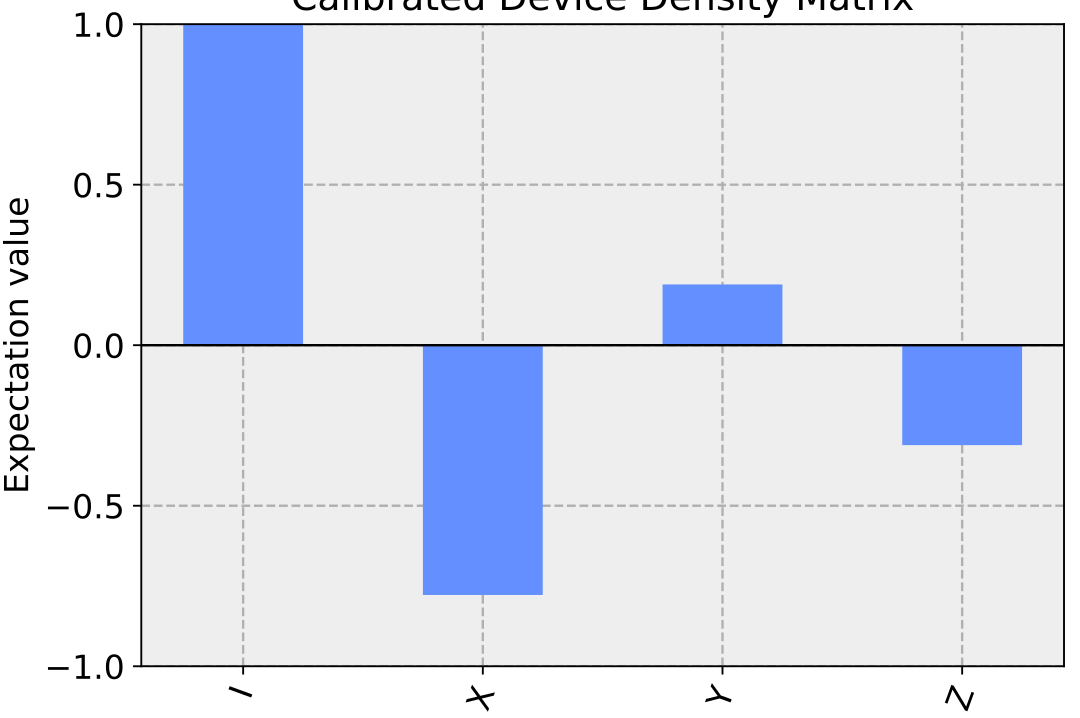
\includegraphics[width=.8\linewidth]{images/results/tele_pauli_cal.png}
    \caption{The calibrated device Pauli set.}
    \label{fig:tele_pauli_dev}
  \end{subfigure}
  \caption{The expectation values match those we expect after calibrating for
readout error. Errors in measurement contribute greatly to the low fidelity of
our final states. The type of correction seen in the figures above accounts for
the increased fidelity for the calibrated device in Fig.
\ref{fig:teleport_histogram}. Data plotted here is taken for 8192 shots on the
Melbourne backend.}
  \label{fig:tele_paulis}
\end{figure}


This thing here is to test a full size picture don't delete.
\begin{figure*}
  \centering
  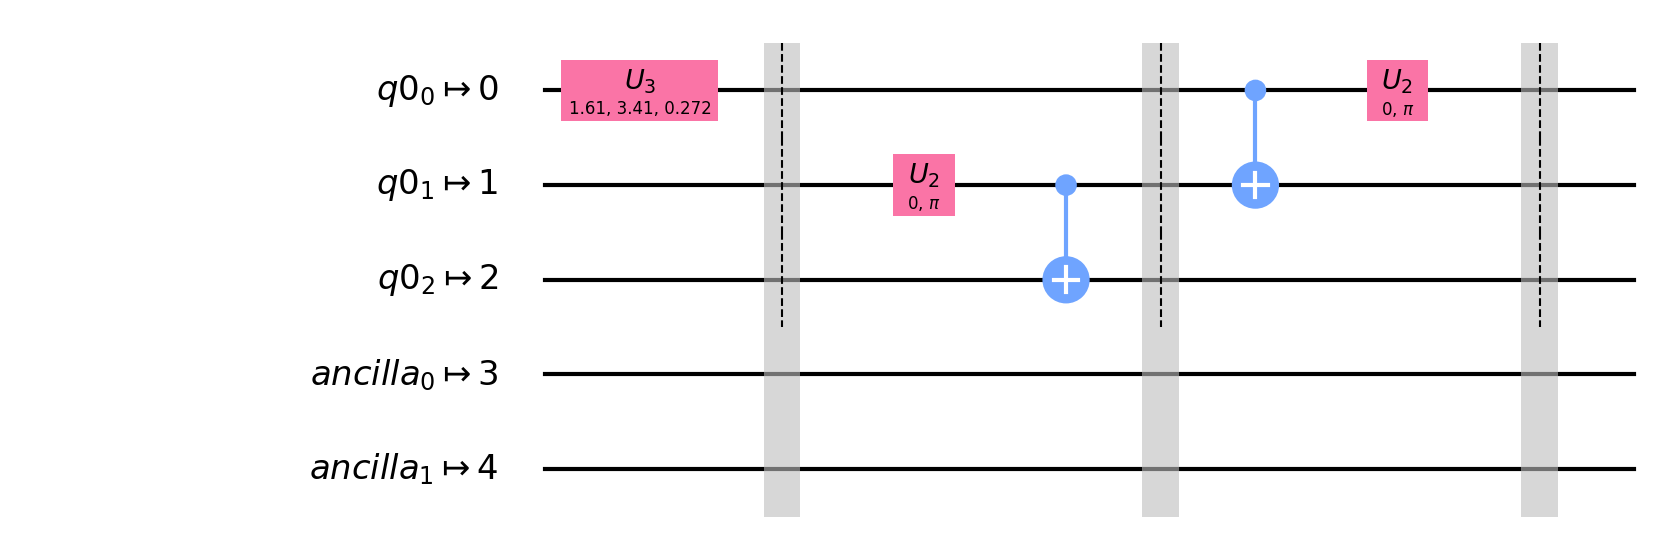
\includegraphics[width=\textwidth]{images/teleport_ibmqx2.png}
  \caption{The most densely connected 5-qubit device at IBM Q. As we will see,
    equally as important as the single-qubit and CNOT error rates is the degree of
    connectivity in a device. Figure from \cite{ibmq_yorktown}.}
  \label{fig:yorktown_connections}
\end{figure*}

\subsection{Entanglement Swapping}
As for teleportation we first look at the main result of the entanglement swapping circuit in Fig. \ref{fig:swap_histogram}. The fidelity measurements are done with a random generated state and a $\ket{\Phi^+}$ Bell-state instead of the regular entanglement swapping circuit where we only swap Bell-states. Again we see that the simulation fidelities are 1 within statistical error, which means that the swapping of initial Bell-states are done correctly using tomography to construct the final state, and post-measurement selection to transform specified results to specific basis. As we expected fidelities from the noisy simulator are much better than results from all the devices. The main difference between teleportation is the fact that Burlington's performance is worse while the other devices give similar (or slightly worse) fidelities. We could predict this behavior since the circuit uses more qubits and hence the total error (due to operations and the qubits themselves) will be more significant. Also note that using the two state tomography method (see Theory) results in an overall improvement of the fidelity. From this phenomena we can conclude that a significant part of the error is due to readout error.   
\begin{figure}[h] \centering
	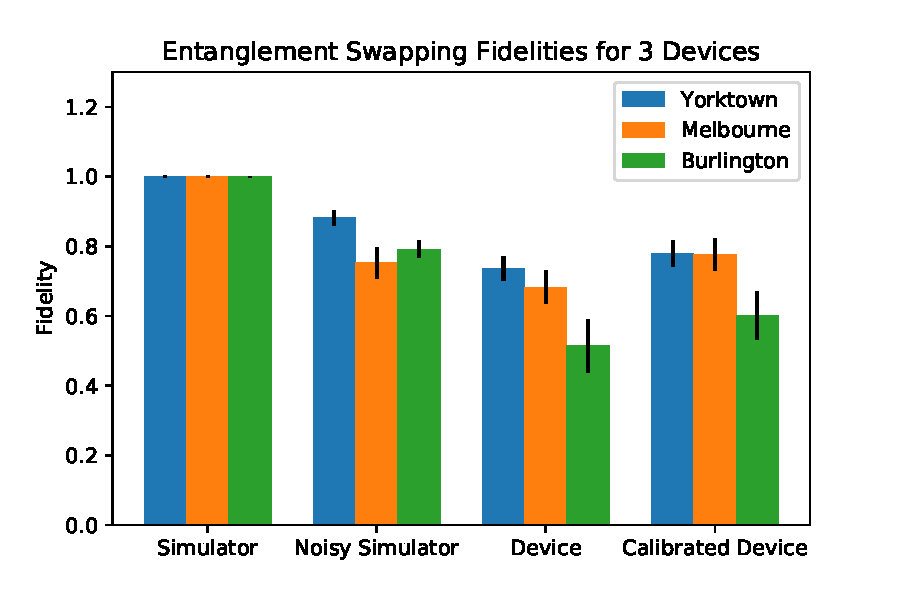
\includegraphics[width=0.48\textwidth]{images/results/swap_histogram.pdf}
	\caption{Fidelity results for the Entanglement Swapping protocol. Error bars are
		estimated by taking the variance over 15 runs of 8,192 shots each (a total of
		122,880 shots).}
	\label{fig:swap_histogram}
\end{figure}

In order to check the readout calibration, it is useful to compare Pauli sets of
the different outcomes, which we can see in Fig. \ref{fig:tele_paulis}.

\begin{figure}
	\begin{subfigure}{.5\textwidth} \centering % include first image
		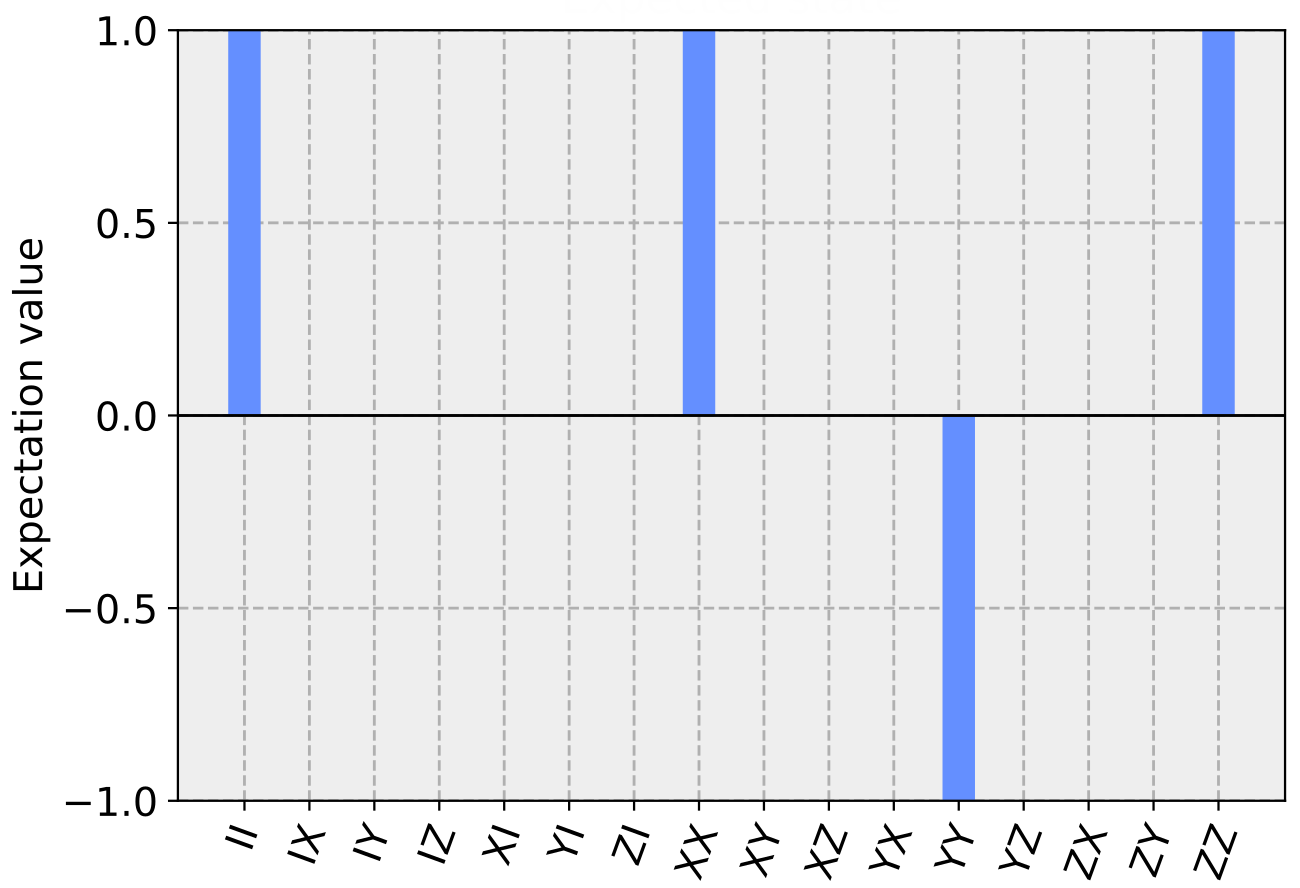
\includegraphics[width=.8\linewidth]{images/results/swap_pauli_sim.png}
		\caption{The expected Pauli set.}
		\label{fig:swap_pauli_sim}
	\end{subfigure} \newline
	\begin{subfigure}{.5\textwidth} \centering % include second image
		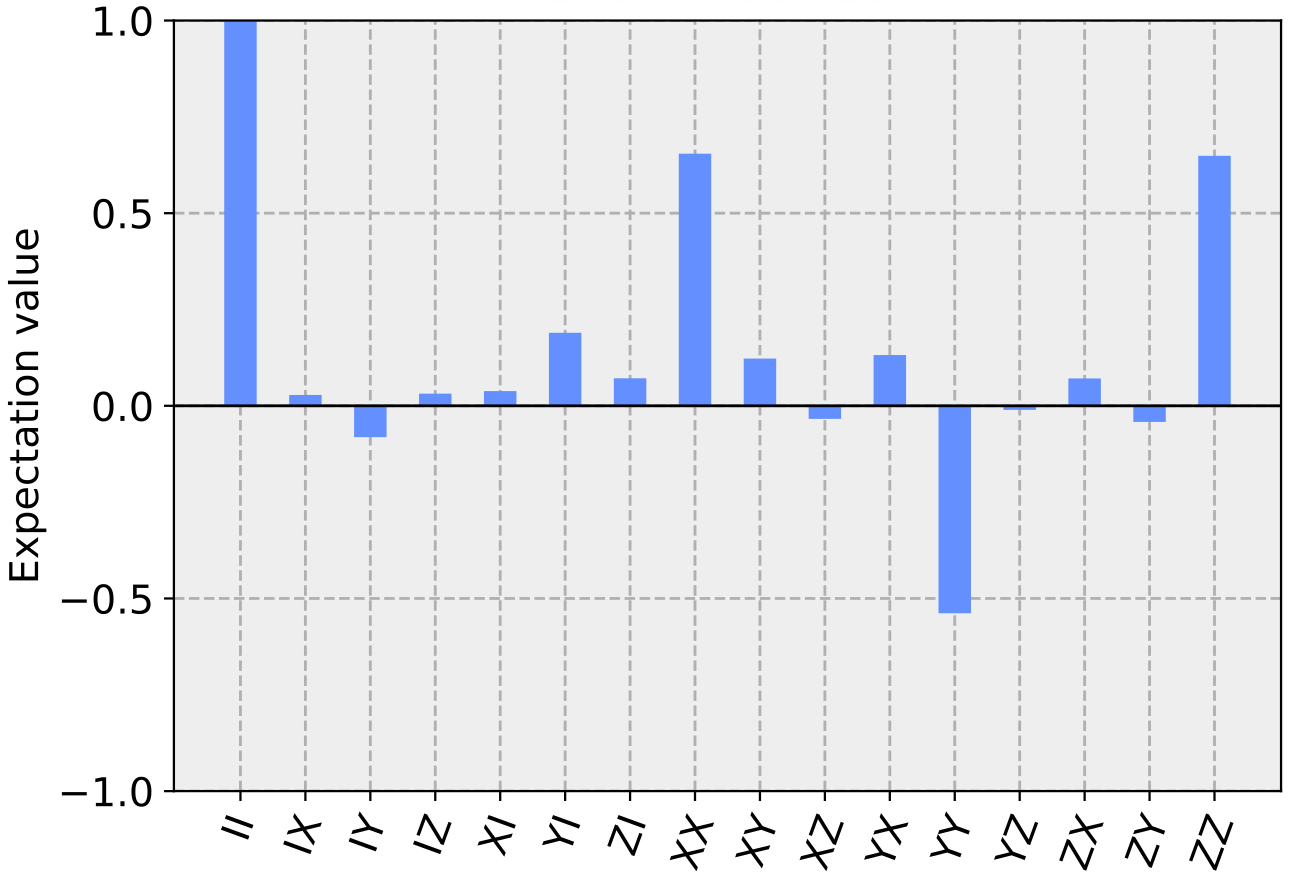
\includegraphics[width=.8\linewidth]{images/results/swap_pauli_dev.png}
		\caption{The output Pauli set for the device.}
		\label{fig:swap_pauli_dev}
	\end{subfigure} \newline
	\begin{subfigure}{.5\textwidth} \centering % include second image
		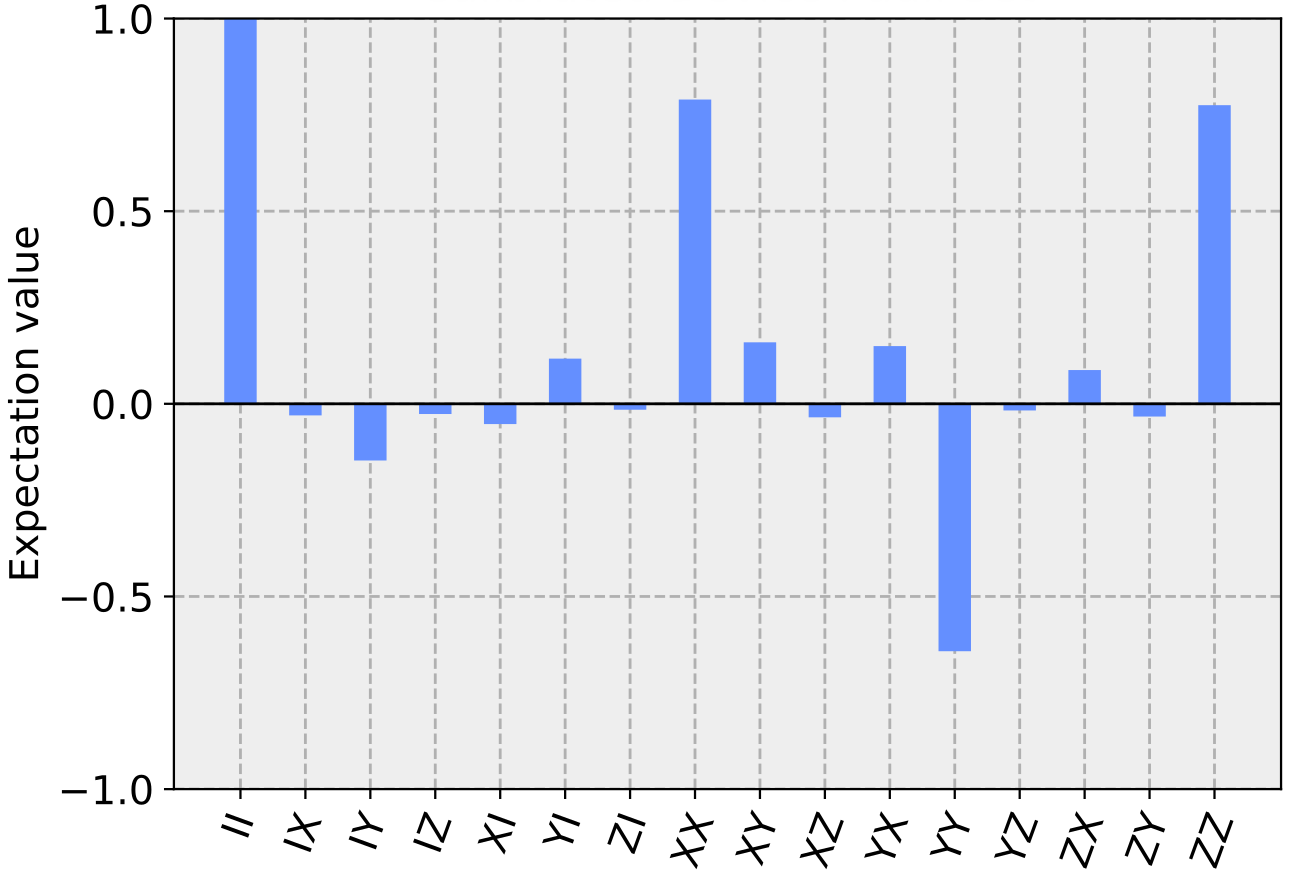
\includegraphics[width=.8\linewidth]{images/results/swap_pauli_cal.png}
		\caption{The calibrated device Pauli set.}
		\label{fig:swap_pauli_dev}
	\end{subfigure}
	\caption{ The type of correction seen in the figures above accounts for
		the increased fidelity for the calibrated device in Fig.
		\ref{fig:swap_histogram}. Data plotted here is taken for 8192 shots on the
		Melbourne backend.}
	\label{fig:tele_paulis}
\end{figure}








\subsection{Entanglement Purification}
\subsection{Grover's Algorithm}


%%% Local Variables:
%%% mode: latex
%%% TeX-master: "report"
%%% End:

\section{Conclusion}

Our research project was mainly focused on the fidelities of different circuits and if we were able to improve those for readout error using state tomography on various circuits. We conclude that we succeeded in recreating the final states using the post measurement method (except for the Grover circuit), since the simulator fidelities for the four circuits are approximately 1. The noisy simulator overestimated the device results for each circuit, and the error correction improves the fidelity for all circuits.  
%%% Local Variables:
%%% mode: latex
%%% TeX-master: "report"
%%% End:

%	REFERENCE LIST
\printbibliography

\section*{Acknowledgements}
We acknowledge use of the IBM Q for this work. The views expressed are those of the authors and do not reflect the official policy or position of IBM or the IBM Q team.

%%% Local Variables:
%%% mode: latex
%%% TeX-master: "report"
%%% End:

\appendix
\section*{Appendix}
  Stuff goes here.


%%% Local Variables:
%%% mode: latex
%%% TeX-master: "report"
%%% End:
\label{apen} % reference to the apendix

\clearpage
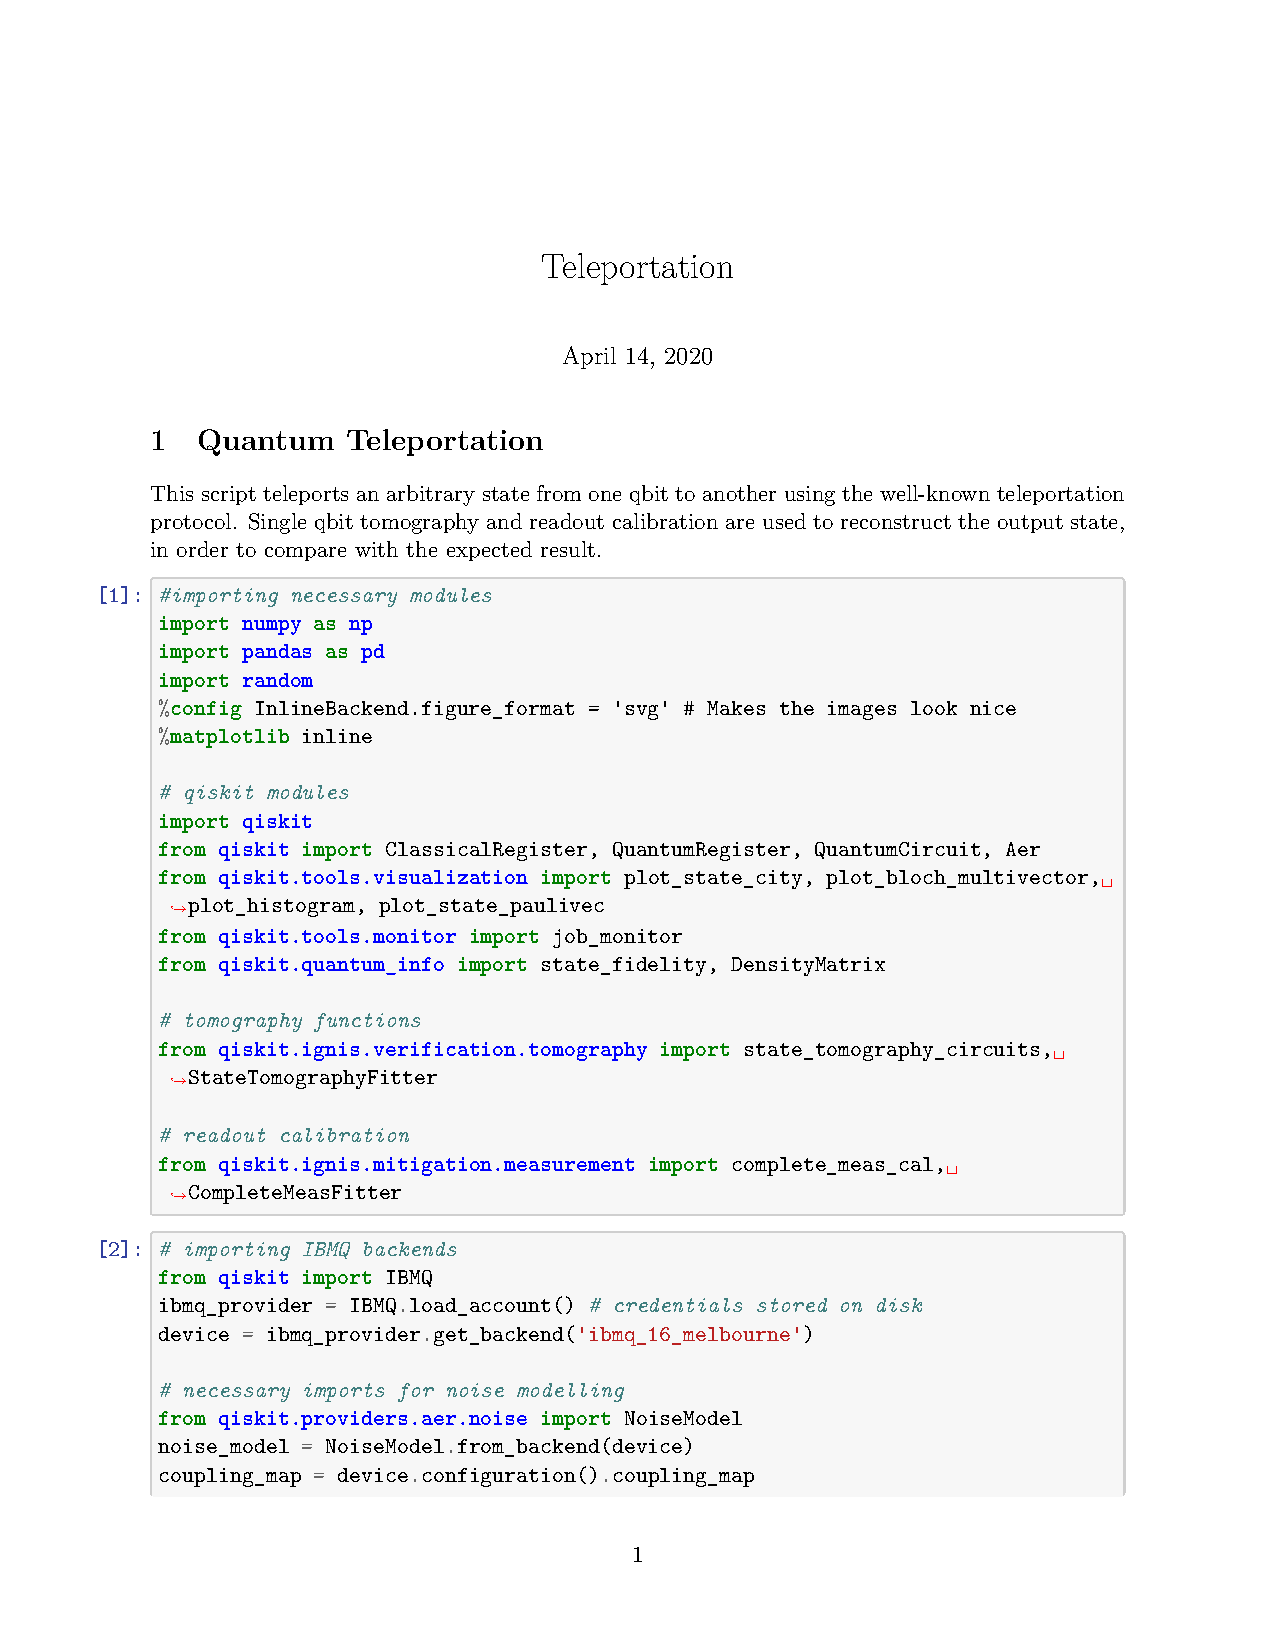
\includepdf[pages=-]{../Circuits/Teleportation.pdf}
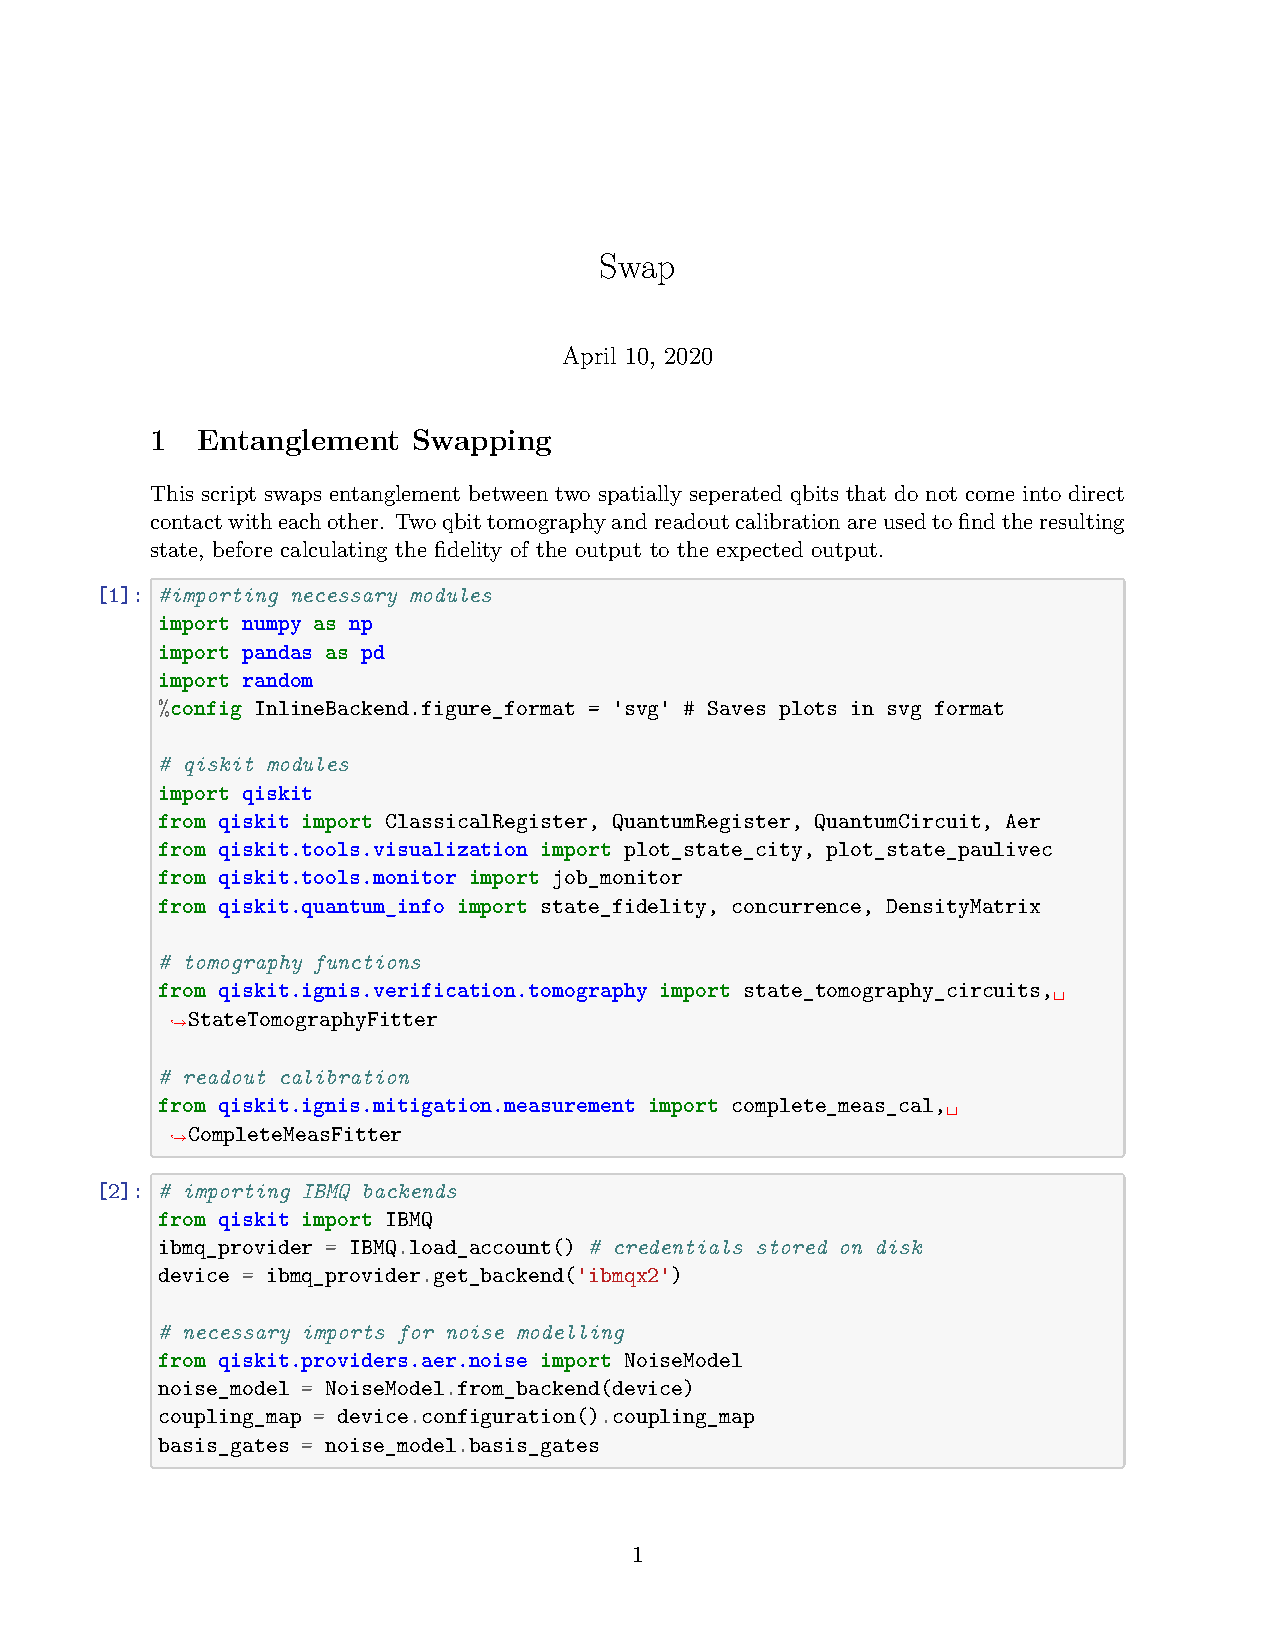
\includepdf[pages=-]{../Circuits/Swap.pdf}
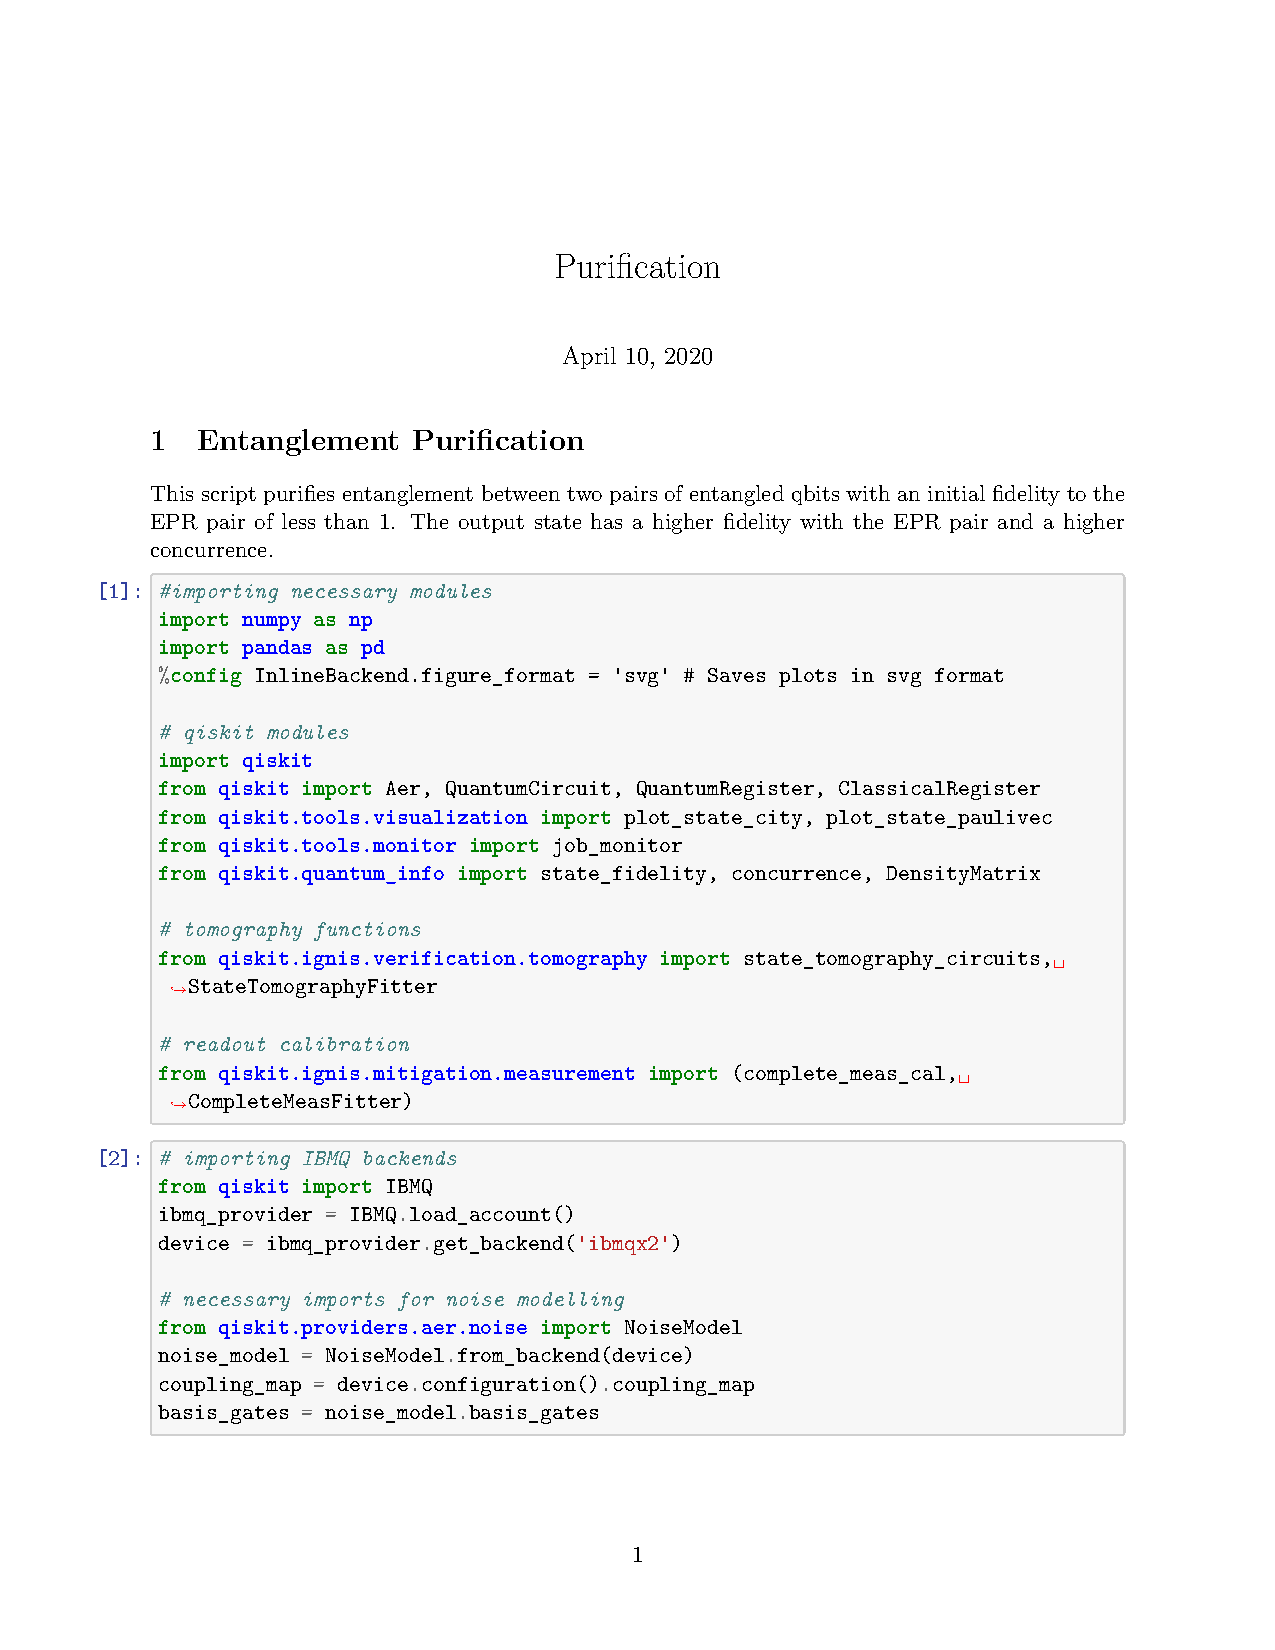
\includepdf[pages=-]{../Circuits/Purification.pdf}
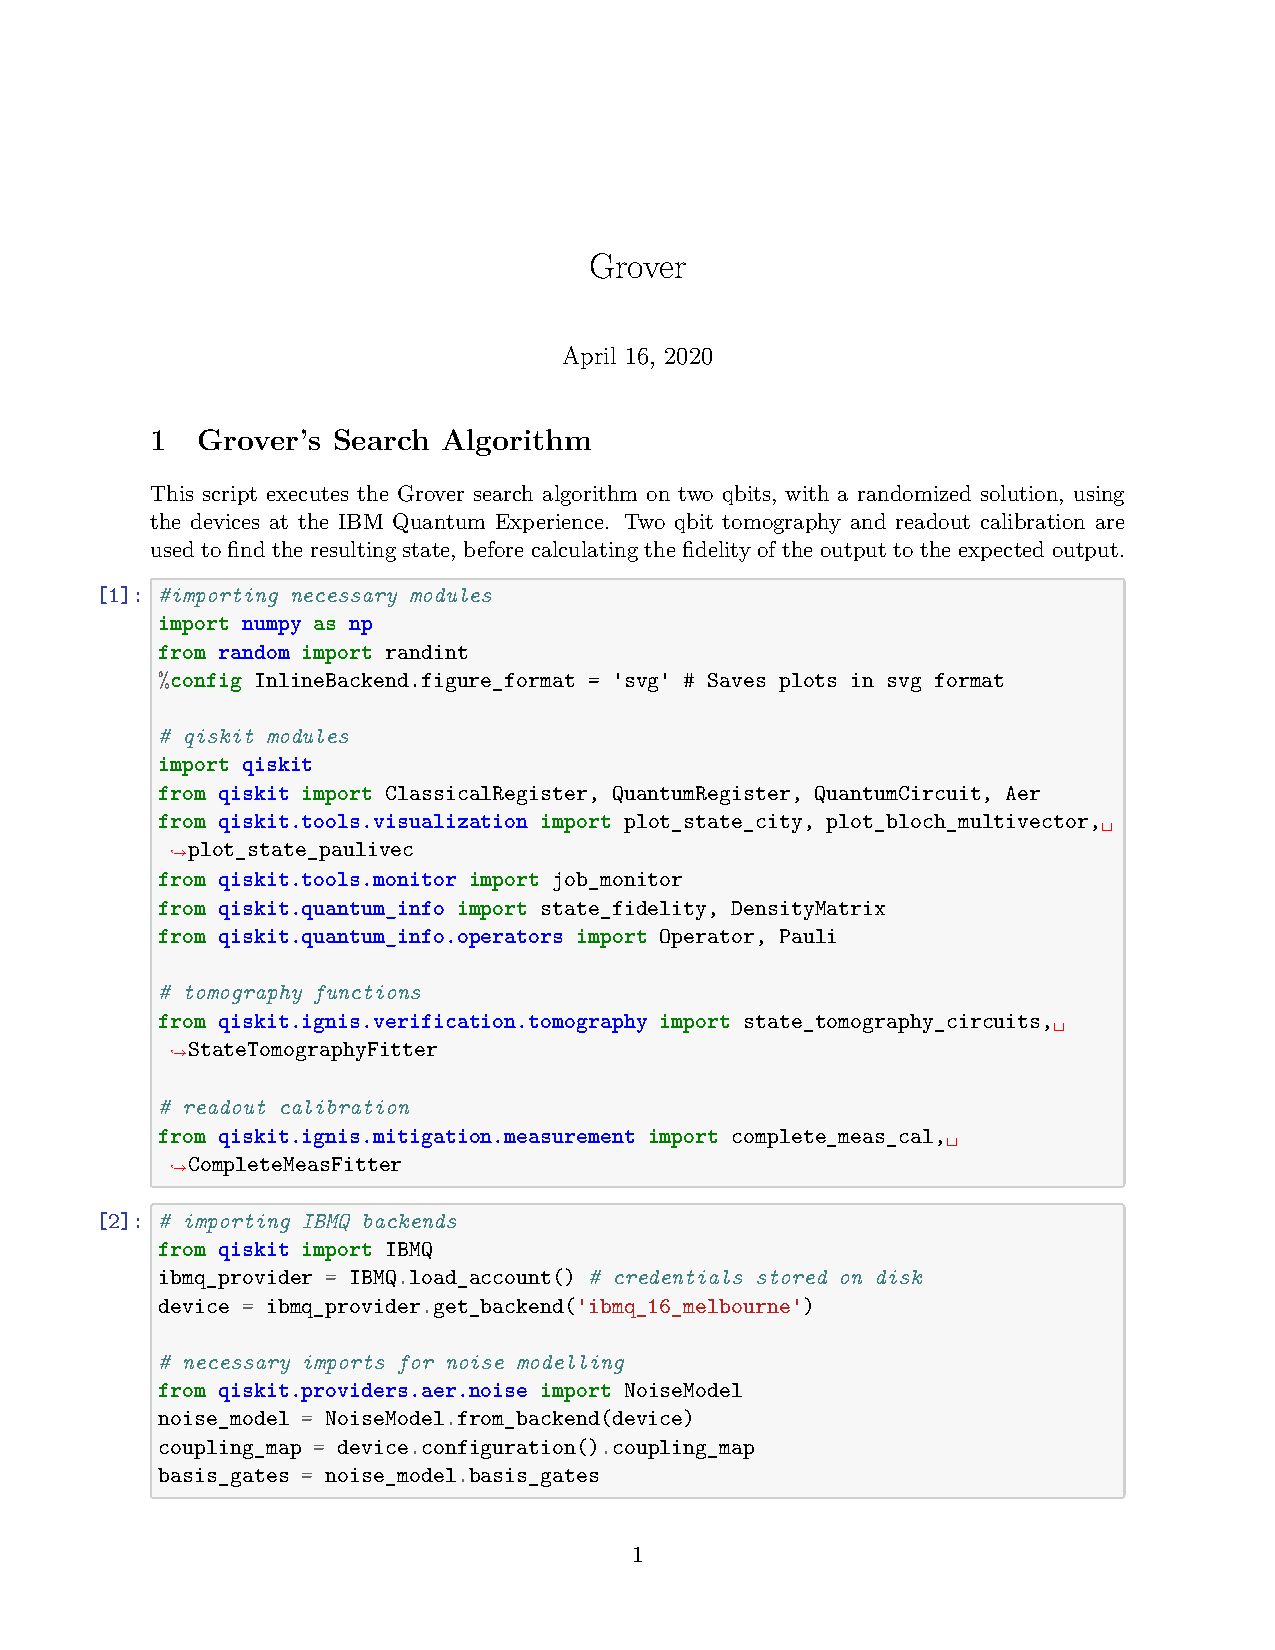
\includepdf[pages=-]{../Circuits/Grover.pdf}

%-----------------------------------------------------------------------------
\end{document}